\usetikzlibrary{arrows.meta,positioning,shapes.geometric, calc}

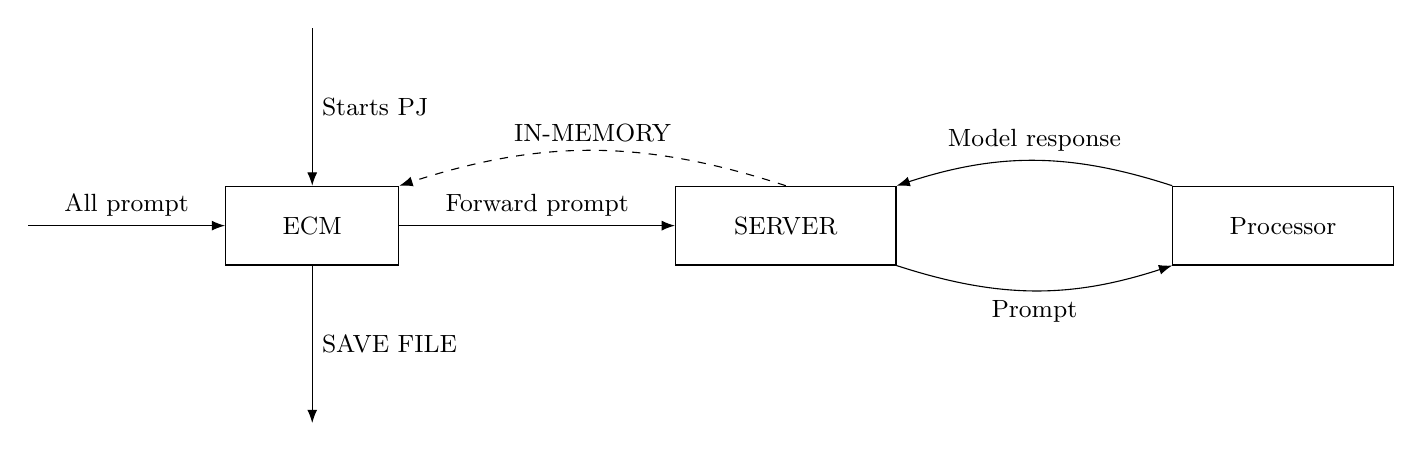
\begin{tikzpicture}[
      >=Latex,
      font=\small,
      node distance=3.5cm,
      ecm/.style   ={rectangle, draw, minimum width=2.2cm,
                     minimum height=1cm, align=center},
      block/.style ={rectangle, draw, minimum width=2.8cm,
                     minimum height=1cm, align=center}
    ]

    \node[ecm] (ecm) {ECM};
    \node[block, right=of ecm] (server) {SERVER};
    \node[block, right=of server] (processor)  {Processor};

    \coordinate[left =2.5cm of ecm] (prompt_in);
    \coordinate[above=2.0cm of ecm] (starts_pj);
    \coordinate[below=2.0cm of ecm] (save_file);

    \draw[->] (prompt_in) -- node[above] {All prompt} (ecm.west);
    \draw[->] (starts_pj) -- node[right] {Starts PJ} (ecm.north);

    \draw[->] (ecm.east) -- node[above] {Forward prompt} (server.west);

    \draw[->, bend right=18] (server.south east) to node[below] {Prompt} (processor.south west);
    \draw[->, bend right=18] (processor.north west) to node[above] {Model response} (server.north east);

    \draw[dashed,->,bend right=18]
          (server.north) to node[above] {IN-MEMORY} (ecm.north east);

    \draw[->] (ecm.south) -- node[right] {SAVE FILE} (save_file);
\end{tikzpicture}